\chapter{Externe Algorithmen}

\begin{minipage}{.6\textwidth}
  Greift man auf sehr große Datenbestände zu, so sind diese in der Regel auf Sekundärspeicher wie Platte oder Band gespeichert, weil diese sehr günstig sind. Problem ist, dass der Zugriff auf den Speicher sehr viel Zeit benötigt.
  
  \term{Externe Algorithmen}\index{Externe Algorithmen} nehmen an, dass die \emph{interne Arbeit}, also die Rechenarbeit, kostenlos ist. Minimiert werden soll die Anzahl an Zugriffen auf den Sekundärspeicher.
\end{minipage}
\hfill
\begin{minipage}{.35\textwidth}
  \begin{figure}[H]
    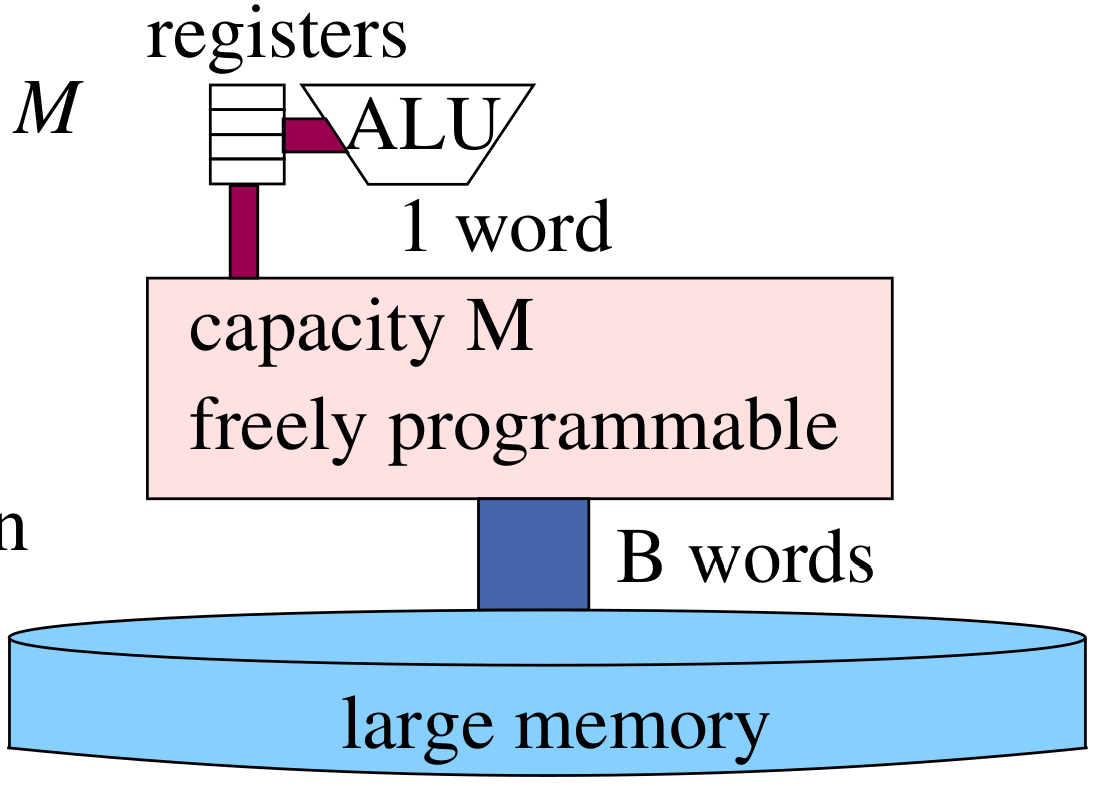
\includegraphics[width=\textwidth]{externalModel}
    \caption{Sekundärspeicher-modell mit schnellem internen Speicher der Größe \( M \) und einem beliebig großem externen Speicher, der über einen \( B \) Wörter breiten Bus angebunden ist}
  \end{figure}
\end{minipage}

\section{Mehrwegemischen}

Als nichttriviales Beispiel werden wir \term{Mehrwegemischen}\index{Mehrwegemischen} betrachten:

\begin{pseudocode}
  \textbf{\textsc{multiwayMerge}}\( (a_1,\dots,a_k,c : \text{File \textbf{of} Element}) \) \\
  \phantom{\enskip} \textbf{for} \( i \coloneqq 1 \) \textbf{to} \( k \) \textbf{do} \( x_i \coloneqq a_i\text{.readElement} \) \\
  \phantom{\enskip} \textbf{for} \( j \coloneqq 1 \) \textbf{to} \( \sum_{i=1}^k \left\vert a_i \right\vert \) \textbf{do} \\
  \phantom{\enskip} \phantom{\enskip} find \( i \in 1\dots k \) that minimizes \( x_i \) \enskip{} \textcolor{gray}{// no IOs, \( O(\log k) \) time} \\
  \phantom{\enskip} \phantom{\enskip} \( c\text{.writeElement}(x_i) \) \\
  \phantom{\enskip} \phantom{\enskip} \( x_i \coloneqq a_i\text{.readElement} \)
\end{pseudocode}

Der Aufwand beträgt

\begin{itemize}
  \item \textbf{I/O}: \( a_i \) lesen \( \approx \frac{\left\vert a_i \right\vert}{B} \), \( c \) schreiben \( \approx \sum_{i=1}^k \frac{\left\vert a_i \right\vert}{B} \)

  \( \Rightarrow \) Insgesamt \( \leq \approx 2\frac{\sum_{i=1}^k \left\vert a_i \right\vert}{B} \)

  \emph{Bedigungung}: brauchen \( k+1 \) Pufferblöcke.

  \item \textbf{Interne Arbeit} durch Benutzung einer Prioritätsliste:
  \begin{equation*}
    O\left( \log k \sum_{i=1}^k \left\vert a_i \right\vert \right)
  \end{equation*}
\end{itemize}

\subsection{Sortieren durch Mehrwegemischen}

Wir können Mehrwegemischen verwenden, um zu sortieren:

\begin{enumerate}
  \item Sortiere \( \left\lceil \tfrac{n}{M} \right\rceil \) runs mit je \( M \) Elementen.
  \item Mische jeweils \( \tfrac{M}{B} \) runs, bis nur noch ein run übrig ist.
\end{enumerate}

Die Anzahl an I/Os setzt sich aus \( 2\tfrac{n}{B} \) I/Os für das sortieren, \( 2\tfrac{n}{B} \) I/Os für das Mischen und \( \left\lceil \log_{M/B} \tfrac{n}{M} \right\rceil \) Mischphasen zusammen, insgesamt also

\begin{equation*}
  \text{sort}(n) \cong \frac{2n}{B}\left( 1 + \left\lceil \log_{M/B} \frac{n}{M} \right\rceil \right) \enskip \text{I/Os.}
\end{equation*}

Die interne Arbeit setzt sich zusmamen aus
\begin{itemize}
  \item run formation: \( O(n\log M) \),
  \item Zugriffe auf die Prioritätsliste pro Phase: \( O\left( n\log \tfrac{M}{B} \right) \),
  \item Anzahl Phasen: \( \left\lceil \log_{M/B} \tfrac{n}{M} \right\rceil \)
\end{itemize}
zusammen, insgesamt

\begin{equation*}
  O\left( n \log M + n\log \tfrac{M}{B} * \left\lceil \log_{M/B} \tfrac{n}{M} \right\rceil \right) = O(n\log n)\text{.}
\end{equation*}